\documentclass[a4paper,10pt]{article}

\usepackage[english,french]{babel}
\usepackage[utf8]{inputenc}
\usepackage[T1]{fontenc}
\usepackage{bookman}
\usepackage{amsmath}
\usepackage{amscd}
\usepackage{amssymb}
\usepackage{amsthm}
\usepackage{latexsym}
\usepackage{graphicx}
\usepackage{color}
\usepackage{calc}
\usepackage[boxruled,vlined,french]{algorithm2e}
\usepackage{setspace}

\setlength{\voffset}{-3.75cm}
\setlength{\hoffset}{-2.6cm}
\setlength{\oddsidemargin}{2.75cm}
\setlength{\topmargin}{2in}
\setlength{\headheight}{0in}
\setlength{\headsep}{0in}
\setlength{\topskip}{0in}
\setlength{\parindent}{0cm}
\setlength{\parskip}{1ex plus0.4ex minus0.2ex}
\setlength{\textwidth}{16.25cm}
\setlength{\textheight}{20.5cm}
\renewcommand{\baselinestretch}{1.5}
\flushbottom
\setcounter{page}{1}
\setcounter{tocdepth}{2}

\SetKw{Edb}{Effet de bord}
\SetKw{Et}{et}
\SetKw{Ou}{ou}
\SetKw{De}{de}
\SetKw{A}{à}
\SetKwBlock{Debut}{Début}{Fin}
\SetKwIF{Si}{SinonSi}{Sinon}{Si}{alors}{Sinon si}{Sinon}{FinSi}
\SetKwFor{Pour}{Pour}{faire}{FinPour}
\SetKwFor{PourTout}{Pour tout}{faire}{FinPour}
\SetKwFor{TantQue}{Tant que}{faire}{FinTantQue}
\SetKw{Retour}{retourner}

\newcommand{\anym}{\emph{anymalign}}
\newcommand{\guill}[1]{« #1 »}

\newtheorem{probleme}{Problème}


% $$$ Faire une Titlepage un peu plus jolie...
\title{ \Large Rapport de stage \\ \LARGE Analyse d'un algorithme d'alignement multilingue}

\author{\normalsize Romain \textsc{Versaevel}, L3 Informatique Fondamentale, ENS de Lyon \\ \normalsize Encadré par M. François \textsc{Yvon}, directeur du LIMSI/CNRS \\}

\date{\today}

\begin{document}

\maketitle

\begin{abstract}
Ce rapport rend compte de mon stage de Licence 3 réalisé au LIMSI/CNRS, durant lequel j'ai étudié l'algorithme d'alignement multilingue \anym .

Après une présentation du domaine de recherche, le traitement automatique des langues parlées, et plus particulièrement la traduction automatique, je propose des résultats pratiques et théoriques qui valident l'algorithme \anym~et en montrent certaines limites. %$$$ LAID
\end{abstract}

\newpage
\tableofcontents
\newpage

\section{Introduction}
J'ai suivi dans le cadre de ma formation, en Licence 3 d'Informatique à l'ENS de Lyon un stage de recherche d'une durée de six semaines, du 2 juin au 11 juillet 2014. Ce stage s'est déroulé au LIMSI (Laboratoire d'Informatique pour la Mécanique et les Sciences de l'Ingénieur), laboratoire CNRS situé sur le campus de l'université Paris-Sud, à Orsay, dans le groupe TLP (Traitement des Langues parlées, ou Spoken Language Processing Group). J'étais encadré par M. François Yvon, directeur du LIMSI.

Le sujet de ce stage était d'analyser l'algorithme d'alignement multilingue \anym, conçu et implémenté par
% $$$
en
% $$$
, et utilisé par le LIMSI pour diverses applications. % $$$

Ce rapport est divisé en quatre parties. Dans la première, je présente le contexte dans lequel s'inscrit mon travail, le domaine de la traduction automatique. Dans la deuxième, je présente l'algorithme que j'ai étudié et l'analyse qui en avait déjà été réalisée. Dans les troisième et quatrième, je présente les résultats de ma propre analyse, empirique (confrontation avec des mesures d'association) et théorique.



\section{Contexte, rappels}

Cette section présente le domaine de recherche dans lequel s'inscrit mon stage : le traitement automatique des langues parlées, puis plus particulièrement la traduction automatique. Elle est essentiellement bibliographique.

\subsection{Traitement des langues parlées}

Le traitement automatique des langues parlées, en anglais \emph{spoken language processing} (ou encore linguistique automatique, \emph{computational linguistics}) est une discipline à l'intersection de l'informatique, de la linguistique, des sciences cognitives. Son objet est l'étude et l'utilisation des langues naturelles avec des outils informatiques.

Ses applications sont nombreuses. On peut citer le traitement du signal pour la simulation et la reconnaissance vocale, les interfaces homme/machine, l'écriture automatique %article du Monde
, et la traduction automatique.

\subsection{Traduction automatique}

La \emph{traduction automatique}, en anglais \emph{machine translation}, a pour objet la traduction de textes d'une langue naturelle vers une autre, par l'intermédiaire d'algorithmes et d'ordinateurs (dans intervention humaine --- on parle sinon de \emph{traduction assistée par ordinateur}). Si l'on peut chercher les origines de cette discipline dans les langues universelles imaginées par Descartes et Leibniz au XVII\textsuperscript{e} siècle
% $$$ ndbdp, citation
, par le truchement desquelles on pourrait passer de n'importe quelle langue à n'importe quelle autre, c'est en 1947 que le mathématicien américain Warren Weaver propose pour la première fois d'utiliser les ordinateurs pour réaliser des travaux de traduction à l'UNESCO.
% http://www.mt-archive.info/Weaver-1947-original.pdf
La discipline a depuis fait des progrès considérables. Ses motivations, développées par John Hutchins dans
%http://www.hutchinsweb.me.uk/PPF-1.pdf
sont nombreuses. Il évoque la nécessité dans certaines professions de consulter des documents rédigés dans des langues très diverses, la simplification de la transmission des savoirs, des applications militaires, mais aussi des raisons plus idéologiques : la traduction permet la communication et donc la paix. Notons que la traduction automatique ne fait pas concurrence aux traducteurs humains, qui s'adressent à un public différent. Sa vocation n'est pas de réaliser des traductions littéraires ou des traductions parfaites, mais de rendre accessible, rapidement et à moindre coût, une très grande quantité de documents à des locuteurs de toutes les langues.

La traduction est un exercice considéré difficile depuis longtemps. \guill{Traduttore, traditore} disent les italiens : \guill{Traduire, c'est trahir}. Les ordinateurs n'ont pas des prétentions si élevées que celle de transmettre fidèlement la pensée de l'auteur original ; ils doivent cependant relever toutes sortes de défis. Ainsi l'idée naïve d'une traduction mot à mot à l'aide d'un simple dictionnaire bilingue produit-elle de très mauvais résultats, parce qu'un mot dans une langue peut se traduire par plusieurs dans une autre (\emph{Rindfleischetikettierungsüberwachungsaufgavenübertragungsgesetz} est ainsi l'équivalent allemand de \emph{loi sur le transfert des obligations de surveillance de l'étiquetage de la viande bovine} en français, soit 1 mot contre 15), parce que la polysémie ou l'homonymie ne sont pas prises en compte (faut-il traduire \emph{avocat} par \emph{avocado} ou \emph{lawyer} ? \emph{cut} par \emph{couper}, par \emph{coupé}, par \emph{coupions} ?), non plus que les idiomes (\emph{Das ist nicht mein Bier} doit être traduit par \emph{Ce ne sont pas mes oignons} et non littéralement par \emph{Ce n'est pas ma bière}), etc.

Bon nombre d'outils de traduction automatique ont été développés, les plus connus étant Google translate et SYSTRAN (utilisé par Yahoo et BabelFish). Les approches sont nombreuses, elles peuvent s'appuyer ou non sur des outils d'analyse linguistique, être unilatérale ou bilatérales, statistiques ou non\dots
% Liens ; statistiques ? $$$

Les algorithmes qui nous intéressent plus particulièrement ici ne sont pas des algorithmes de traduction pure mais des algorithmes d'\emph{alignement}, qui génèrent des données pour les premiers en analysant des corpus édités en plusieurs langues. On cite souvent l'exemple de Champollion qui apprit à déchiffrer les hiéroglyphes grâce à la pierre de Rosette. Les algorithmes d'alignement utilisent ainsi des corpus multilingues --- dont il existe grâce à Internet de grandes quantités --- pour en extraire des relations de traduction entre des paires de mot. Le plus utilisé est Giza++.

%@misc{och2003giza++,
%  title={GIZA++},
%  author={Och, FJ},
%  year={2003}
%}

% Berkeley Word Aligner, Nile, ...

% Le stage que j'ai effectué portait sur l'analyse d'un algorithme d'alignement par échantillonnage, \anym, développé par Adrien Lardilleux.


\subsection{Quelques définitions et notations}

Avant d'étudier plus avant \anym, il convient de poser quelques définitions.

Dans un texte en langue naturelle, on appelle \emph{segment} (\emph{phrase} en anglais) un ensemble de mots. On appellera en outre $n$-gramme un segment de $n$ mots consécutifs.

On appelle \emph{corpus multilingue} un ensemble de textes en plusieurs langues. On appelle \emph{corpus parallèle} un corpus multilingue dont les textes sont traduction les uns des autres. Enfin, un corpus parallèle est \emph{aligné} lorsque sont déterminées des relations (de traduction) entre segments de ses textes.

\anym~considère des corpus parallèles de taille arbitraire alignés au niveau des phrases, et construit un dictionnaire d'alignements de segments plus petits. On limitera ici notre analyse à des corpus de deux seulement textes, qu'on appellera \emph{texte source} et \emph{texte cible}
% ; un mot ou segment du texte source sera généralement noté $e$ (comme \emph{english}) et du texte cible $f$ (comme \emph{french} ou \emph{foreign})
.

%@article{Brown:1990:SAM:92858.92860,
% author = {Brown, Peter F. and Cocke, John and Pietra, Stephen A. Della and Pietra, Vincent J. Della and Jelinek, Fredrick and Lafferty, John D. and Mercer, Robert L. and Roossin, Paul S.},
% title = {A Statistical Approach to Machine Translation},
% journal = {Comput. Linguist.},
% issue_date = {June 1990},
% volume = {16},
% number = {2},
% month = jun,
% year = {1990},
% issn = {0891-2017},
% pages = {79--85},
% numpages = {7},
% url = {http://dl.acm.org/citation.cfm?id=92858.92860},
% acmid = {92860},
% publisher = {MIT Press},
% address = {Cambridge, MA, USA},
%} 




\section{Présentation d'\emph{anymalign}}

\subsection{L'algorithme}

\subsubsection{(bis)}

\begin{algorithm}
\setstretch{1.5}
\caption{anymalign \label{algoanym}}

\SetKwData{g}{g}\SetKwData{arbre}{arbre}\SetKwData{nun}{n1}\SetKwData{ndeux}{n2}\SetKwData{nbN}{g.nbN}\SetKwData{ares}{ares}
\SetKwData{Cu}{C$_1$}
\SetKwData{Cn}{C$_n$}
\SetKwData{Wu}{w$_{n_1}$}
\SetKwData{Wn}{w$_{n_k}$}
\SetKwData{AlC}{Alignements}
\SetKwData{iii}{i}
\SetKwData{jjj}{j}
\SetKwData{www}{w}
\SetKwData{J}{J}
\SetKwData{I}{I}
\SetKwData{Sub}{S}
\SetKwData{Profils}{Profils}
\SetKwFunction{ajouter}{ajouter}
\Entree{Corpus parallèle $(\Cu, \dots, \Cn)$.}
\Sortie{Table d'alignements \AlC.}

\Debut
{
	\Pour{\iii de $1$ à \I}
	{
		\Sub $\leftarrow$ sous-corpus de taille $|\Sub|$

		\Pour{\jjj de $1$ à \J}
		{
			\PourTout{\jjj-gram \www dans \Sub}
			{
				Calculer son profil (vecteur de présence) \\
				\ajouter$(\www,\Profils)$
			}

			\PourTout{profil dans \Profils}
			{
				\PourTout{groupe de mots $(\Wu,\dots,\Wn)$}
				{

					$\AlC[(\Wu,\dots,\Wn)]$ ++
				}
			}
		}
	}
	\Retour \AlC
}
\end{algorithm}

La fonction auxiliaire $ajouter$ incorpore le mot $w$ dans la table $Profils$, initialement vide, de telle sorte que :

\begin{itemize}
\item si $Profils$ contient déjà $w'\subset w$ de même profil que $w$, alors $w'$ est écrasé par $w$ ;
\item si plusieurs segments d'un même texte ont le même profil, ils sont finalement tous rejetés.
\end{itemize}

% Mouais, c'est globalement moyen. $$$

\subsubsection{Exemple}
% $$$ Exemple !!

\subsubsection{Remarques}
% Raffinement n-grams

Tel que présenté ici, l'algorithme termine après $I$ itérations ; en réalité, dans l'implémentation qui en a été faite, de nombreuses conditions d'interruption différentes peuvent être utilisées : après un certain temps, lorsque le nombre d'alignements par secondes devient inférieur à une certain borne, ou encore par une interruption manuelle de l'utilisateur.

\anym~est comme on le voit un algorithme statistique, dont l'exécution ne dépend pas de la taille du corpus ; il  utilise les seuls textes parallèles (et aucune donnée linguistique) ; c'est en outre un algorithme complètement symétrique : tous les corpus $C_i$ jouent le même rôle. Pour cette raison, on peut se contenter pour l'analyse de deux corpus $C_1$ et $C_2$, mais il s'agit évidemment d'une qualité importante de l'algorithme.


\subsection{Qualités et défauts}
(L'analyse déjà réalisée)


\section{Mesures d'association}

Dans cette section, après avoir introduit la notion de \emph{mesure d'association} en statistiques, je compare les résultats empiriques fournis par \anym~avec différentes mesures d'association classiques.

\subsection{Topo sur les mesures d'association}

En statistiques, on appelle \emph{mesure d'association} une relation entre plusieurs variables aléatoires non-indépendantes. Le terme est proche de celui de \emph{corrélation} même si ce dernier a une définition plus contrainte, impliquant notamment d'un \emph{facteur de corrélation}.

En théorie de l'information, il s'agit le plus souvent de comparer deux variables aléatoires $X$ et $Y$. Notons $e$ et $f$ les événements $X \in E$ et $Y \in F$. Les mesures d'association entre $X$ et $Y$ utiliseront généralement les valeurs de la table de contingence ($\mathfrak{F}(e)$ désigne la fréquence absolue de l'événement $e$ dans un effectif de taille totale $N$) :

\begin{tabular}{|cc|c|}
\hline
$a := \mathfrak{F}(e\wedge f)$ & b := $\mathfrak{F}(e\wedge\overline{f})$ & $\mathfrak{F}(e)$ \\
$c := \mathfrak{F}(\overline{e}\wedge f)$ & $d := \mathfrak{F}(\overline{e}\wedge\overline{e})$ & $\mathfrak{F}(\overline{e})$ \\
\hline
$\mathfrak{F}(f)$ & $\mathfrak{F}(\overline{f})$ & $N$ \\
\hline
\end{tabular}

Ici, $X$ et $Y$ seront des mots ; $E$ et $F$ désigneront les phrases alignées d'un corpus parallèle de taille $N$. On mesurera donc l'association de deux mots à travers la probabilité qu'ils apparaissent dans les mêmes phrases ($a$), le premier mais pas le deuxième ($b$), etc.

Les mesures utilisées sont listées dans le tableau suivant (les noms sont donnés en anglais car certains n'ont pas d'équivalent français) :

\begin{tabular}{|l|l|}
\hline
Nom & Formule \\
\hline
Likelihood ratio ou $G^2$ &
 $2\left(a\log\left(\frac{aN}{(a+b)(a+c)}\right) +b\log\left(\frac{bN}{(a+b)(b+d)}\right) +c\log\left(\frac{cN}{(a+c)(c+d)}\right) +d\log\left(\frac{dN}{(b+d)(c+d)}\right)\right)$ % $$$
\\

Pointwise % $$$ ?
 mutual information (PMI)  & $\log_2(\frac{aN}{(a+b)(a+c)})$ \\

%& $\sum_{x=e,\overline{e}}\sum_{y=f,\overline{f}}\mathfrak{F}(x\wedge y)\log\left(\frac{\mathfrak{F}(x\wedge y)}{\mathfrak{F}(x)\mathfrak{F}(y)}\right)$ \\

$\Phi^2$ de Church \& Gale & $\frac{(ad-bc)^2}{(a+b)(a+c)(b+d)(c+d)}$ \\

Coefficient $Q$ de Yule & $\frac{ad-bc}{ad+bc}$ \\

Coefficient $\omega$ de Yule & $\frac{\sqrt{ad}-\sqrt{bc}}{\sqrt{ad}+\sqrt{bc}}$ \\

% Odds ratio & $\frac{ad}{bc}$ \\

Jaccard & $\frac{a}{a+b+c}$ \\

Normalized expectation & $\frac{2a}{2a+b+c}$ \\
%+redondant Jaccard?

Salience & $\log\left(\frac{aN}{(a+b)(a+c)}\right)\cdot\log(a)$  \\
% redondant PMI?

t test & $\frac{a-\frac{(a+b)(a+c)}{N}}{\sqrt{a(1-\frac{a}{N})}}$ \\   %$$$

z score & $\frac{a-\frac{(a+b)(a+c)}{N}}{\sqrt{\frac{(a+b)(a+c)}{N}(1-\frac{(a+b)(a+c)}{N^2})}}$ \\ %$$$

Braun-Blanquet & $\frac{a}{\max(a+b,a+c)}$ \\

Simpson & $\frac{a}{\min(a+b,a+c)}$ \\

Laplace & $\frac{a+1}{\min(b,c)+a+2}$ \\

\hline
\end{tabular}

% Viennent de [] et [] $$$
% Equivalences [] $$$

On constate une grande diversité dans ces mesures, permise par la définition assez laxiste. Le principe est que la mesure est d'autant plus élevée que les les variables aléatoires sont dépendantes suivant un certain schéma. Notre objectif est de montrer que les paires de mots fréquemment alignées par \anym~ont une association forte. Il s'agit donc de comparer deux mesures d'association, puisque \anym~en réalise aussi une, quoique plus compliquée que les précédentes. En effet, le rapport du nombre de fois qu'un couple de mots est aligné par le nombre d'itérations converge vers la probabilité que ce couple ait le même profil dans un sous-corpus tiré aléatoirement.

\subsection{Comparaison avec \anym}

Dans cette partie, on compare les résultats d'\anym~ avec les mesures d'association listées précédemment.

\subsubsection{\anym}

Ces résultats ont été obtenus en traitant un corpus français-anglais de 1000 lignes extrait d'Europarl % $$$
. L'exécution d'\anym~a été interrompue après de 2 200 000 itérations ; le nombre de nouveaux alignements par seconde était alors inférieur à 1 ; un peu plus de 45 000 paires de mots ont ainsi été alignées.

Les paires les plus alignées correspondent aux mots-outils, très fréquents :

\begin{tabular}{|l|l|l|}
\hline
Français & Anglais & Nombre d'alignements \\
\hline
. & . & 6185271 \\
et & and & 394766 \\
je & I & 330634 \\
rapport & report & 329316 \\
Commission & Commission & 286020 \\
concurrence & competition & 277991 \\
\hline
\end{tabular}

Les alignements erronés les plus fréquents font eux aussi intervenir des mots-outils, présents dans une grande majorité des phrases ; le premier d'entre eux est (\guill{.},\guill{the}), au 103\textsuperscript{e} rang avec 25031 alignements.

1451 mots sont alignés plus de 1000 fois, 8266 mots plus 100 fois, 28264 mots plus de 10 fois.

Le critère de comparaison qui a été retenu pour comparer \anym~aux autres mesures d'association est le nombre d'alignements produits. % D'autres ont été envisagées (notamment le \emph{score}) $$$

\subsubsection{Jaccard}

L'une des mesures d'association produisant les meilleurs résultats est le Jaccard dont on rappelle l'expression : $Jacc(e,f)=\frac{a}{a+b+c}=\frac{\mathfrak{F}(e\wedge f)}{\mathfrak{F}(e\wedge f)+\mathfrak{F}(e\wedge\overline{f})+\mathfrak{F}(\overline{e}\wedge f)}$ ou, si l'on note $E$ (resp. $F$) l'ensemble des phrases où apparaît $e$ (resp. $f$) : $Jacc(e,f)=\frac{E\cap F}{E\cup F}$.

La figure \ref{jaccard} montre le nombre d'alignements % échelle log
 réalisés par \anym~en fonction du Jaccard. On y observe une association importante : 
% Il faudrait peut-être étoffer ça d'une régression linéaire ? Je ne sais pas faire...
pour $j$ fixé, les couples de mots de Jaccard proche de $j$ les plus alignés le sont d'un nombre proche de $C\cdot j$ ($C$ une constante, ici égale à % $$$
, mais qui est de peu d'importance puisqu'elle dépend de la durée d'exécution de l'algorithme.) Ainsi, l'absence de points dans les coins supérieur gauche (les paires d'association faible sont peu alignées) et inférieur droit (les paires de forte association sont beaucoup alignées) valident l'algorithme.

En revanche, l'épaisseur de la courbe, en d'autres termes le grand nombre de points situés en-dessous de la courbe $y = C\cdot x$ montre une variation importante dans les alignements réalisés par \anym~pour des mots de même Jaccard
% $$$ quantifier ça...

\begin{figure}[t]
\centering
\label{jaccard}
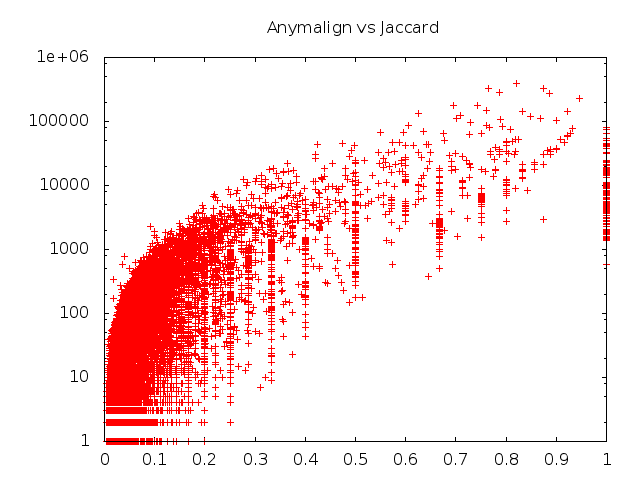
\includegraphics[width=12cm]{jacclog.png} % $$$ Penser à relooker (plus grand, échelle log au lieu de log, pas "../../moy/...")
\caption{LEGENDE} % $$$
\end{figure}

Ces résultats montrent une ressemblance importante entre les résultats d'\anym~et le Jaccard ; l'algorithme en donne une estimation
% $$$ je ne sais décidément pas chiffrer ces choses-là...
% $$$ glisser une remarque sur la complexité (échantillonnage versus n²)
On aurait cependant espéré une proximité encore supérieure : la motivation de ces travaux se trouve dans % [] Broder, à expliquer.

% Autres mesures qui donnent un résultat proche (Annexe) : Braun-Blanquet, Laplace, Normalized expectation, Simpson, t test $$$

\subsubsection{PMI}
% Du coup je ne sais pas vraiment ce que c'est !!
% \log_2(Na/((a+b)(a+c))) = log_2(P(xy)/(P(x)P(y)))

L'une des mesures d'association produisant les meilleurs résultats est l'Information Mutuelle (IM) % $$$
 Jaccard dont on rappelle l'expression : $IM(e,f)=\log_2\left(\frac{aN}{(a+b)(a+c)}\right)=\log_2\left(\frac{\mathfrak{F}(e\wedge f)\cdot N}{\mathfrak{F}(e)\cdot\mathfrak{F}(f)}\right)$ (avec $N$ la taille totale du corpus).

La figure \ref{jaccard} montre le nombre d'alignements % échelle log
 réalisés par \anym~en fonction du Jaccard. On y observe une association importante : 
% Il faudrait peut-être étoffer ça d'une régression linéaire ? Je ne sais pas faire...
pour $j$ fixé, les couples de mots de Jaccard proche de $j$ les plus alignés le sont d'un nombre proche de $C\cdot j$ ($C$ une constante, ici égale à % $$$
, mais qui est de peu d'importance puisqu'elle dépend de la durée d'exécution de l'algorithme.) Ainsi, l'absence de points dans les coins supérieur gauche (les paires d'association faible sont peu alignées) et inférieur droit (les paires de forte association sont beaucoup alignées) valident l'algorithme.

\begin{figure}[t]
\centering
\label{im}
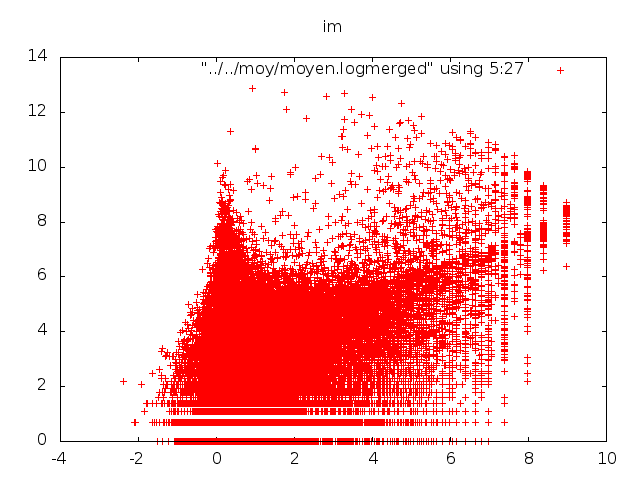
\includegraphics[width=12cm]{imlog.png} % $$$ Penser à relooker (plus grand, échelle log au lieu de log, pas "../../moy/...")
\caption{LEGENDE} % $$$
\end{figure}

% \begin $$$
- Dépend trop de la fréquence (mots rares à droite, mot fréquents à gauche).

- A droite : log(N)=9,96 ; mots rares équivalents % $$$ il faudra dire que ça te tient pas compte des hapaxes !...

- 0 et en-dessous : mots assez fréquents mais sans intérêt. Malheureusement, beaucoup d'alignements juste au-dessus de 0...

- Les bons alignements entre mots fréquents sont entre 1 et 4 ; les bons alignements moyen

- Bilan : sans invalider l'algorithme, le pic autour de 0 trahit la présence importante de "déchet"

% \end $$$

% Autres mesures qui donnent un résultat proche (Annexe) : Rawim (?), Yule's omega, Yule's Q, Salience $$$

\subsubsection{Conclusion}

% Autres mesures qui ne donnent que des fichus résultats $$$


\section{Analyse théorique}

Dans cette partie, on cherche à analyser \anym~à l'aide de quelques calculs de probabilités.

La notion qu'il m'a paru intéressant d'étudier est celle de profil, qui est intrinsèquement liée au fonctionnement d'\anym.

On considère un sous-corpus quelconque $S$, composé de $|S|$ phrases parallèles dont on fera l'hypothèse simplificatrice qu'elles sont toutes de longueur $m$. Soient $\Pi$ un profil (c'est-à-dire un élément de $\{0;1\}^{|S|}$), et $w$ un mot de fréquence $\varphi$.

Notons $\mathcal{P}_{w,\Pi}$ la probabilité que $w$ ait le profil $\Pi$ dans $S$
% \footnote{On s'intéresse ici aux paramètres $f$ et $|\Pi|$ ; il pourra être intéressant par la suite d'étudier les variations de la taille du corpus, $|S|$ et $m$.}
. La longueur des phrases étant constante, elle ne dépend que de $|\Pi|$ ; c'est la probabilité que $w$ apparaisse au moins une fois dans exactement $|\Pi|$ des $|S|$ phrases du sous-corpus. En faisant l'hypothèse que les mots sont tirés au hasard d'après leur seule fréquence, la probabilité que $w$ n'apparaisse pas dans une phrase donnée est $(1-\varphi)^m$ et donc

\begin{align*}
\mathcal{P}_{w,\Pi} & = (1-\varphi)^{m(|S|-|\Pi|)} \cdot (1-(1-\varphi)^m)^{|\Pi|} \\
				& = (1-\varphi)^{m|S|}\cdot\left[(1-\varphi)^{-m}-1\right]^{|\Pi|}
\end{align*}

Soient maintenant $w$ et $w'$ deux mots de fréquences respectives $\varphi$ et $\psi$. Notons $\mathcal{A}_{w,w'}$ la probabilité que ces deux mots aient le même profil et $\check{\mathcal{A}}_{w,w'}$ la probabilité que ces deux mots aient le même profil \emph{non-nul} dans $S$.

On a alors sous \emph{l'hypothèse que $w$ et $w'$ sont indépendants} :

\begin{align*}
\mathcal{A}_{w,w'} & = \sum_{\Pi~profil}\mathcal{P}_{w,\Pi}\cdot\mathcal{P}_{w',\Pi} \\
				& = \sum_{\Pi~profil}(1-\varphi)^{m|S|}\cdot((1-\varphi)^{-m}-1)^{\Pi} \cdot(1-\psi)^{m|S|}\cdot((1-\psi)^{-m}-1)^{\Pi} \\
				& = \sum_{\Pi~profil}[(1-\varphi)(1-\psi)]^{m|S|}\cdot[((1-\varphi)^{-m}-1)((1-\psi)^{-m}-1)] \\
				& =~~ \sum_{k=0}^{|S|}~\sum_{|\Pi|=k} [(1-\varphi)(1-\psi)]^{m|S|}\cdot[((1-\varphi)(1-\psi))^{-m}-(1-\varphi)^{-m}-(1-\psi)^{-m}+1]^{|\Pi|} \\
				& =~~ \sum_{k=0}^{|S|}\binom{|S|}{k} [(1-\varphi)(1-\psi)]^{m|S|}\cdot[((1-\varphi)(1-\psi))^{-m}-(1-\varphi)^{-m}-(1-\psi)^{-m}+1]^k \\
				& =~~ [(1-\varphi)(1-\psi)]^{m|S|} \cdot[((1-\varphi)(1-\psi))^{-m}-(1-\varphi)^{-m}-(1-\psi)^{-m}+2]^{|S|} \\
				& =~~ [1-(1-\varphi)^m-(1-\psi)^m+2(1-\varphi)^m(1-\psi)^m]^{|S|}
\end{align*}

et

\begin{align*}
\check{\mathcal{A}}_{w,w'} & =~~ \sum_{\Pi\neq 0}\mathcal{P}_{w,\Pi}\cdot\mathcal{P}_{w',\Pi} \\
					& =~~ \sum_{k=1}^{|S|}\binom{|S|}{k} [(1-\varphi)(1-\psi)]^{m|S|}\cdot[((1-\varphi)(1-\psi))^{-m}-(1-\varphi)^{-m}-(1-\psi)^{-m}+1]^k \\
					& =~~ [(1-\varphi)(1-\psi)]^{m|S|}\cdot[[((1-\varphi)(1-\psi))^{-m}-(1-\varphi)^{-m}-(1-\psi)^{-m}+2]^{|S|}-1] \\
					& =~~ [1-(1-\varphi)^m-(1-\psi)^m+2(1-\varphi)^m(1-\psi)^m]^{|S|} - [(1-\varphi)(1-\psi)]^{m|S|}
\end{align*}

% $$$ ?
% set logscale
% splot [0.0001:0.1] [0.0001:0.1] ((1-((1-x)**20)-((1-y)**20)+2*((1-x)**20)*((1-y)**20))**15)-(((1-x)*(1-y))**300)


\subsection{Alignement de e et f}

Soient $e$ et $f$ deux mots de deux langues différentes (de fréquences respectives $\varphi$ et $\psi$). On va supposer que toutes les phrases du corpus ont une longueur $20$ et qu'\anym~sélectionne des sous-corpus de taille $|S|=15$. L'espérance du nombre d'alignements de $e$ et $f$ en $k$ étapes est $\mathbb{E}[Al(e,f)] \leq k\check{\mathcal{A}}_{e,f}$ (l'inégalité vient du fait qu'avoir le même profil non-nul est une condition nécessaire mais pas suffisante pour que $e$ et $f$ soient alignés : il faut aussi qu'ils soient les seuls dans leur langue respective à posséder ce profil).

Ainsi, si l'on suppose l'indépendance de $e$ et $f$, que $k=10^6$, et que $\varphi = \psi$ (ce qui maximise % un mot plus propre que "localement" ? $$$
$\check{\mathcal{A}}_{e,f}$), on obtient les  soit $\mathbb{E}[Al(e,f)] \leq 27210$.

\begin{tabular}{|l|l|l|}
\hline
$\varphi$ & $\mathbb{E}[Al(e,f)] \leq \dots$ & \anym \\
\hline
\end{tabular}

% Je confronte quoi avec quoi idéalement ?... $$$

\subsection{Alignement de n-grams}

\subsection{Autres pistes}


\section{Conclusion}


\section{Bibliographie}

\bibliographystyle{plain}
\bibliography{mabiblio}

\section{Annexes}

% Autres figures $$$

\end{document}

% Où parlé-je de Zipf ? $$$









% $$$
%\section{Autres pistes}
%\subsection{Chinois}
%\subsection{Vitesse de convergence}
%\subsection{Discussion sur la taille du sous-corpus} +m
%\subsection{generateur.c}


